The Silicon Vertex Tracker (SVT) is the key detector of the HPS experiment for measuring particle momentum and trajectories through a magnetic field in order to reconstruct the invariant mass and the vertex position of the $e+e-$ pair. The SVT is composed of six layers of 0.7$\%$ radiation length-thick silicon placed downstream of the target and housed in a vacuum chamber within the analyzing magnet. The SVT is separated into top and bottom halves with a 15~mrad opening angle and the first layer of the SVT at $\pm$0.5~mm from the active beam. A drawing of the SVT is shown in Figure~\ref{Figure:svt}.

\begin{figure}[H]
  \centering
      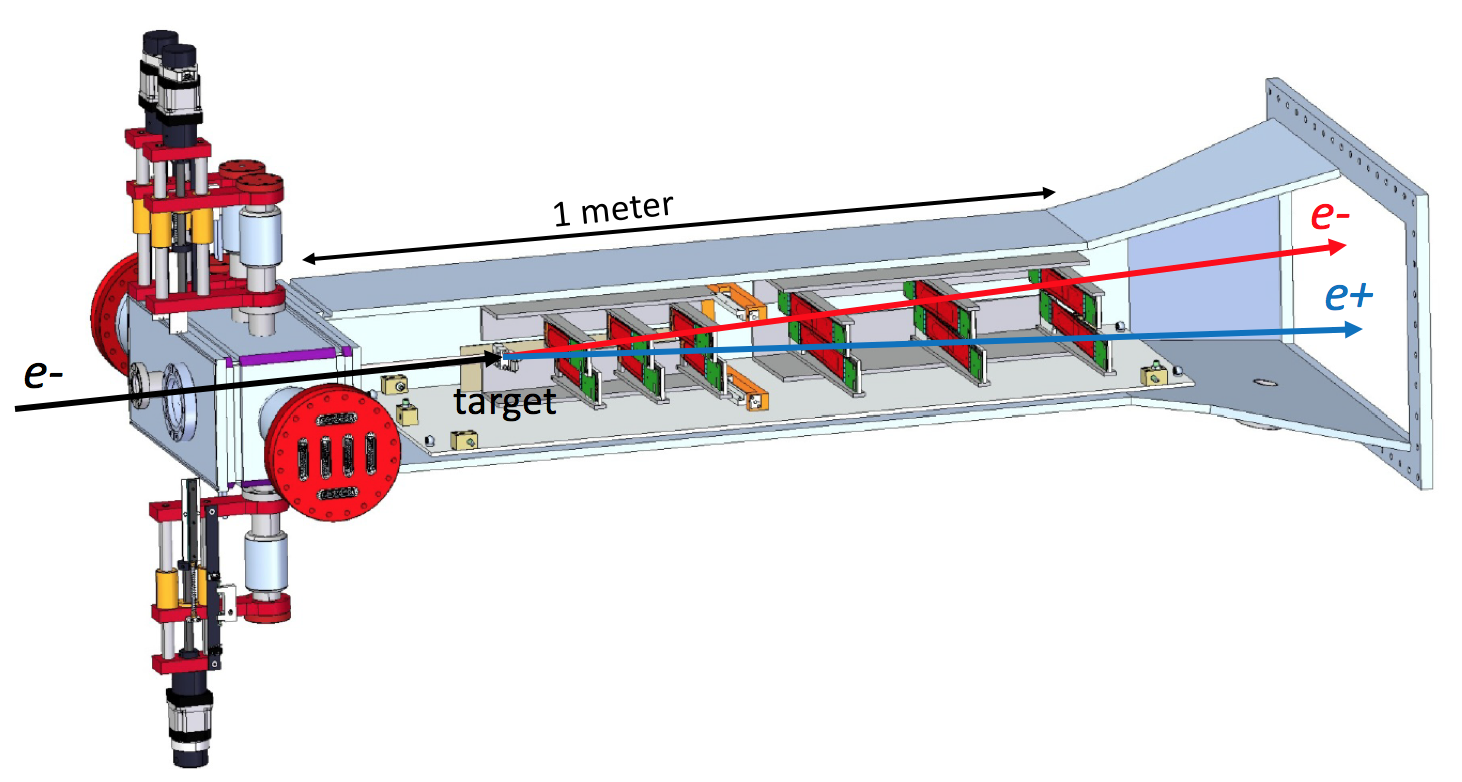
\includegraphics[width=1.0\textwidth]{pics/experiment/svt.png}
  \caption[Rendering of the HPS SVT]{A rendering of the HPS SVT. The beam enters from the left through the vacuum box. The silicon sensors are shown in red, and the hybrid readout boards are shown in green.}
  \label{Figure:svt}
\end{figure}


The SVT, as shown in Figure~\ref{Figure:svt}, is housed in a magnetic field such that particles are bent horizontally (field acts downward). Each of the six layers is composed of two strips capable of measuring a hit position in one dimension. By setting the strips at a stereo angle with respect to one another, each layer of the SVT is capable of three-dimensional hit reconstruction. The first three layers of the SVT are one silicon strip sensor-wide and have a stereo angle of 100~mrad between the strips. The last three layers of the SVT are two strip sensors-wide in order to better match the Ecal acceptance. The stereo angle between the sensors in layers four through six is 50~mrad. The axial sensors are oriented along the bend plane direction whereas the stereo sensors are angled with the lower end closer to the beam plane on the positron side where the background are less intense. The different stereo angles are used to eliminate ghost hits that can generate ghost tracks. The first five layers of the SVT cover the Ecal acceptance while the sixth layer has a slightly reduced acceptance but can be used to improve track reconstruction. The full track reconstruction only requires five hits per track in order to pick up tracks that may be missing hits due to an inefficiency. \\
\indent The hybrid readout boards on each sensor house the APV25 readout chips that connect the sensor to the data acquisition (DAQ) system. The power to the APV25 chips is supplied through the hybrid, and the temperature of the strip is also actively monitored at the hybrid. The heat generated by the operating hybrid is pulled out through the aluminum support structure. As the sensors are cooled for operation, the support structure and sensor contract at slightly different rates. In order to adjust and maintain the sensor at a constant tension, one end of the sensor is attached to a spring pivot in order to maintain rigidity. The assembly of a silicon sensor is shown in Figure~\ref{Figure:svtAssembly}.
\begin{figure}[H]
  \centering
      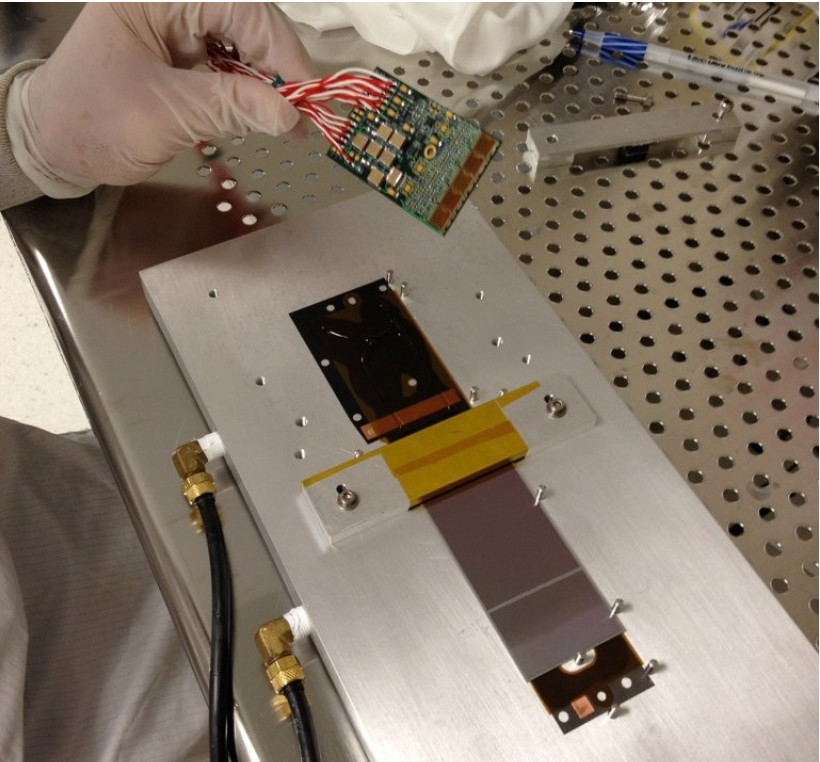
\includegraphics[width=0.5\textwidth]{pics/experiment/svtSensorAssembly.png}
  \caption[Assembly of a half module of the SVT ]{A half module is being assembled for Layers 1-3 of the SVT. A readout hybrid with the APV25 chips is being attached to the frame along the silicon sensor.~\cite{Proposal}}
  \label{Figure:svtAssembly}
\end{figure}
The APV25 samples the strips every 24~ns and stores the results in a pipeline. Once a trigger is received, the corresponding channel pipeline is readout. The readout yields six samples at 24~ns intervals that can be fit to reconstruct the waveform. A 4-pole functional fit was used to extract the time and amplitude of the corresponding hit. A latency time that is configured in the SVT DAQ is used to correctly determine which channel pipelines are readout that correspond to the trigger. The latency time is approximately equal to the time delay of the trigger. Some early data in the Engineering Run was lost due to incorrectly timing in the SVT latency. 
